\documentclass[aspectratio=169,10pt]{beamer}

\usetheme{metropolis}
\usepackage{appendixnumberbeamer}

\usepackage{booktabs}
\usepackage[scale=2]{ccicons}

\usepackage{pgfplots}
\usepgfplotslibrary{dateplot}

\usepackage{xspace}
\newcommand{\themename}{\textbf{\textsc{metropolis}}\xspace}

\usepackage{graphicx}
\usepackage{fontspec}
\usepackage{setspace}
\usepackage{listings}
\usepackage{amsmath}

% Uses Ethereum colorful logo instead of bullet, for all item levels.
\defbeamertemplate{itemize item}{image}{\large
\includegraphics[height=1.6ex]{images/bullet}}
\defbeamertemplate{itemize subitem}{image}{\large
\includegraphics[height=1.6ex]{images/bullet}}
\defbeamertemplate{itemize subsubitem}{image}{\large
\includegraphics[height=1.6ex]{images/bullet}}
\setbeamertemplate{itemize item}[image]
\setbeamertemplate{itemize subitem}[image]
\setbeamertemplate{itemize subsubitem}[image]


% Sets the template background image for all the slides.
% Change opacity here.
\setbeamertemplate{background}{%
	\begin{tikzpicture}[remember picture,overlay]
		\node[at=(current page.center),opacity=0.2]{
			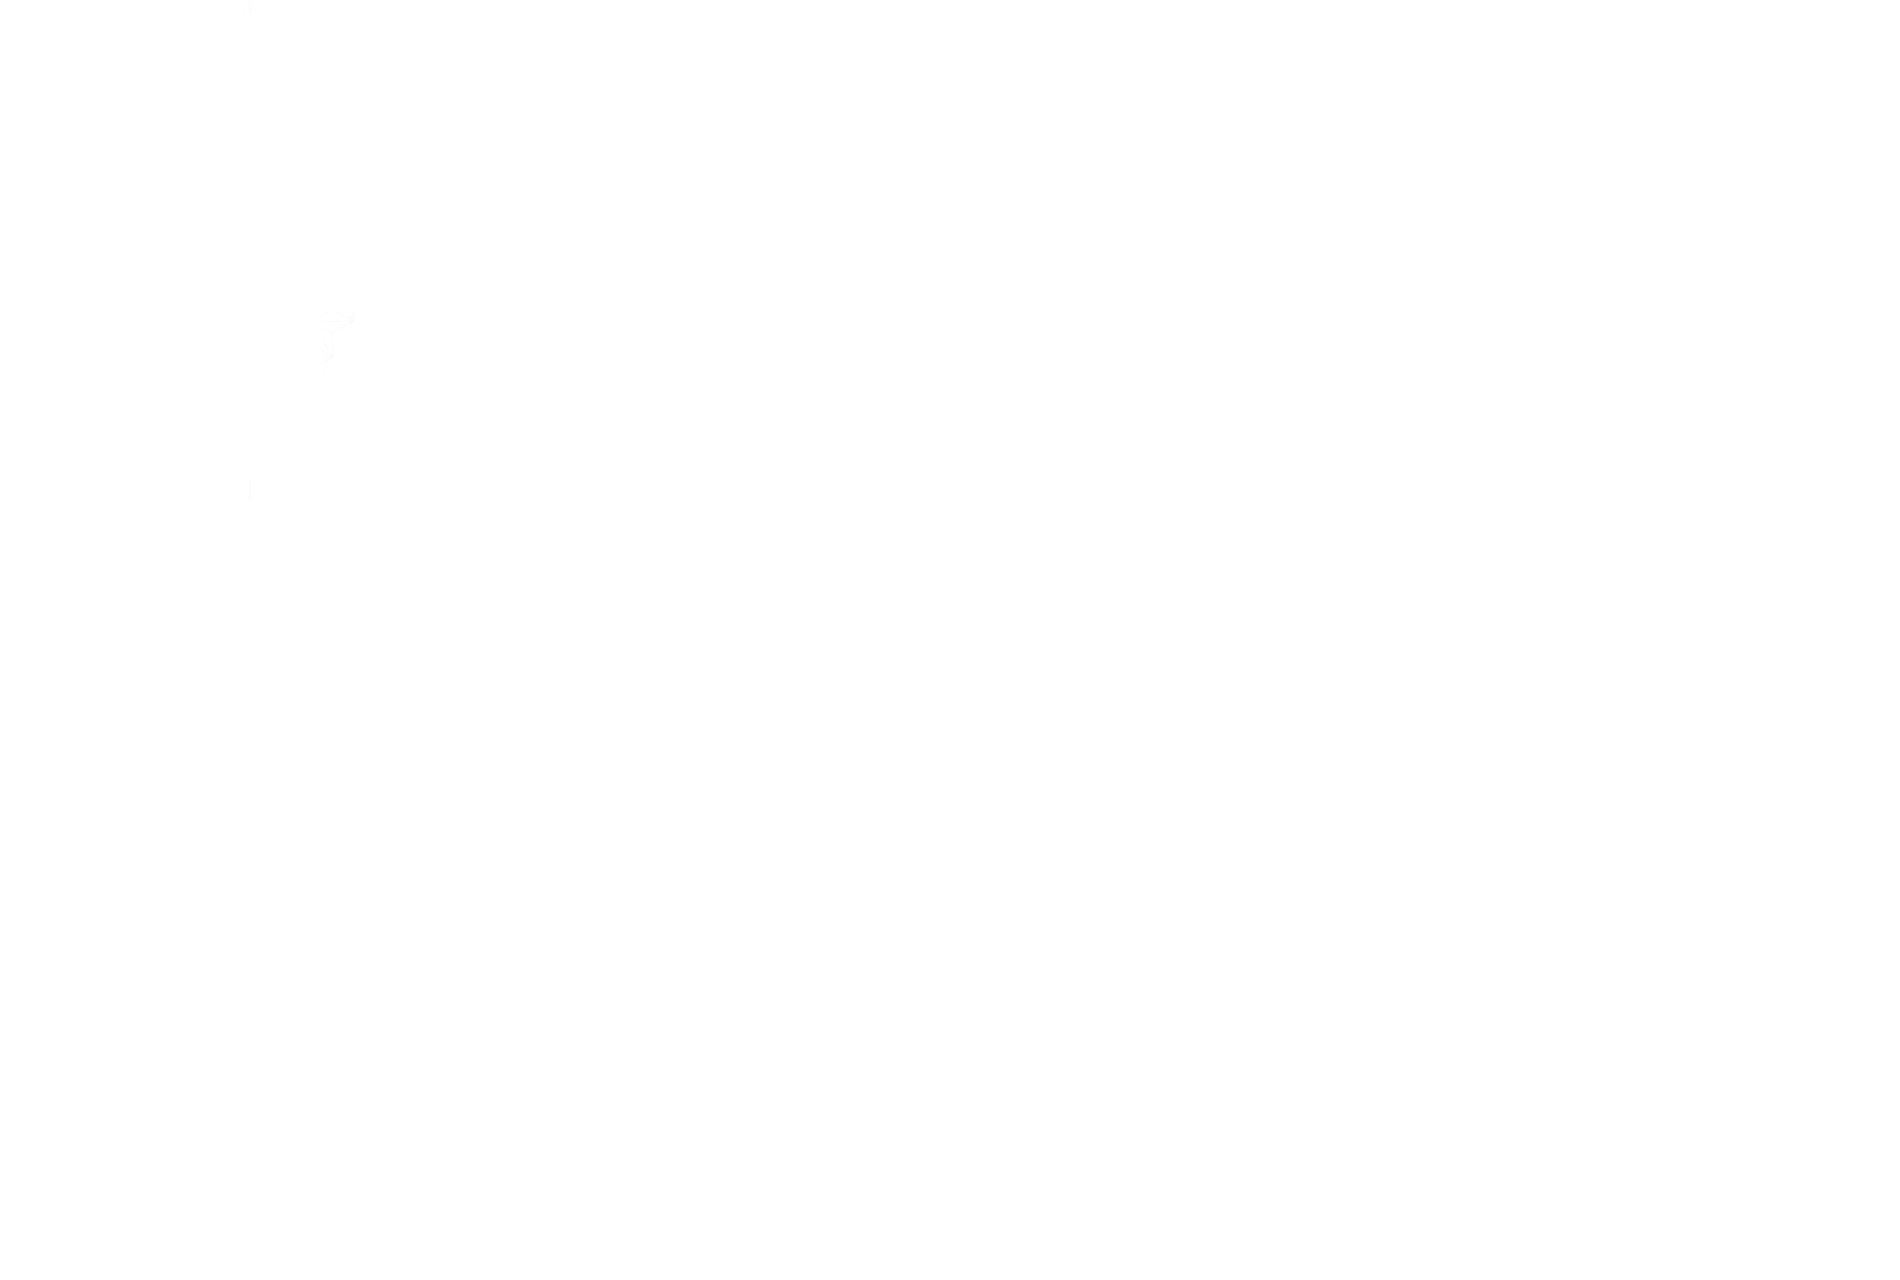
\includegraphics[width=\paperwidth,height=\paperheight]{images/bg}
		};
	\end{tikzpicture}
}


% Sets the color theme.
% Change here for light theme.
% `sectionpage=none` removes slide between sections.
%\metroset{background=dark,sectionpage=none}
%\metroset{background=light}
\metroset{background=dark}
\usebeamercolor[fg]{normal text}

% Sets the footer `devcon v` on the bottom right.
% Change `devcon v` text color here.
\setbeamercolor{frame footer}{fg=gray}
\setbeamertemplate{frame footer}{devcon v}

% Sets the new fonts.
\setsansfont{Circular Std Bold}
\setmonofont{Overpass Mono}

% Sets the default line spacing.
\setstretch{1.5}

% Sets monospace font for tables and quotes.
\AtBeginEnvironment{table}{\ttfamily}
\AtBeginEnvironment{quote}{\ttfamily}
\AtBeginEnvironment{figure}{\ttfamily}

% Sets the normal text font as monospace.
\setbeamerfont{normal text}{family=\ttfamily}
\AtBeginDocument{\usebeamerfont{normal text}}

% If you use the light theme, you need to manually change the
% icons to `_black`.
% Change your GitHub username here.
\setbeamertemplate{github}{
  \small
\includegraphics[height=1.6ex]{icons/github_white}
  \texttt{leonardoalt}
}
% Change your email here.
\setbeamertemplate{email}{
  \small
\includegraphics[height=1.6ex]{icons/email_white}
  \texttt{leo@ethereum.org}
}
% Change your twitter account here.
\setbeamertemplate{twitter}{
  \small
\includegraphics[height=1.6ex]{icons/twitter_white}
  \texttt{leonardoalt}
}

% Remove here any contact you do not want to show.
\setbeamertemplate{contact}{
  \vspace*{2mm}
  \usebeamertemplate{github}\\
  \usebeamertemplate{email}\\
  \usebeamertemplate{twitter}
}

% Change presentation data here.
\title{{\huge Fully automated inductive invariants inference for Solidity smart contracts}}
\author{{\large Leonardo Alt}}
% Change date here.
% Empty date removes it from the frame.
% \date{\today} prints compilation date.
%Otherwise prints content.
\date{} %\date{\today}
\institute{{\large Ethereum Foundation}}
% Sets the Ethereum/devcon logo on the upper left.
\titlegraphic{\vfill
\includegraphics[height=1.2cm]{images/devcon}}

\lstdefinelanguage{Solidity}{
  keywords={break, continue, new, do, while, for, if, else, true, false, return, returns, msg, tx, block, this, require, assert, revert, throw},
  morecomment=[l]{//},
  morecomment=[s]{/*}{*/},
  morestring=[b]',
  morestring=[b]",
  ndkeywords={contract, import, pragma, bool, uint, public, internal, view, pure, payable, using, function},
  keywordstyle=\color{mLightBlue}\bfseries,
  ndkeywordstyle=\color{mLightRed}\bfseries,
  identifierstyle=\color{mAlmostWhite},
  commentstyle=\color{mLightPurple}\ttfamily,
  stringstyle=\color{mLightPink}\ttfamily,
  sensitive=true
}

\begin{document}

{
\setbeamertemplate{background}{%
	\begin{tikzpicture}[remember picture,overlay]
		\node[at=(current page.center),opacity=0.1]{
			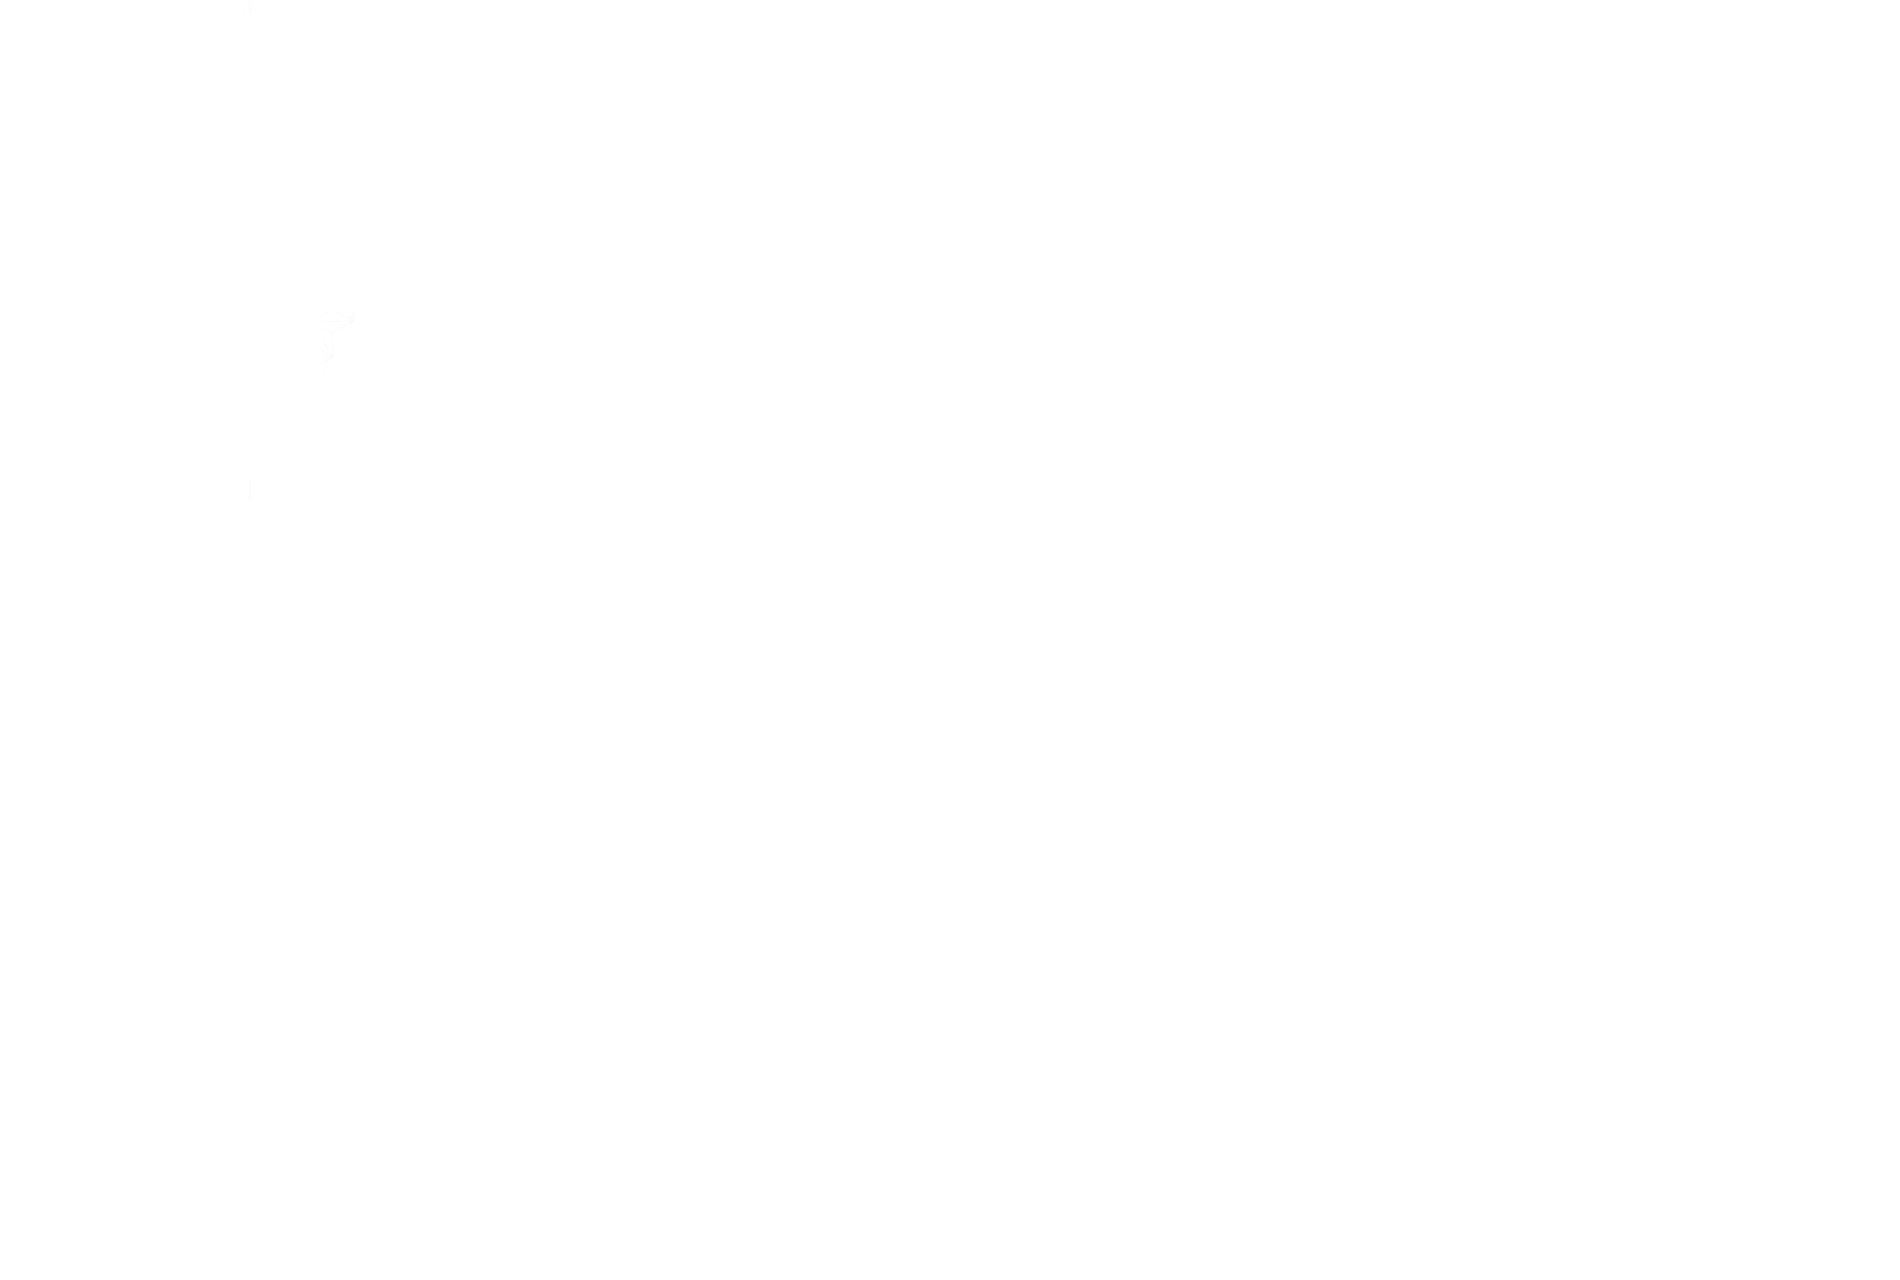
\includegraphics[width=\paperwidth,height=\paperheight]{images/bg}
		};
		\node[opacity=0.9] at (11.5,-2) {
			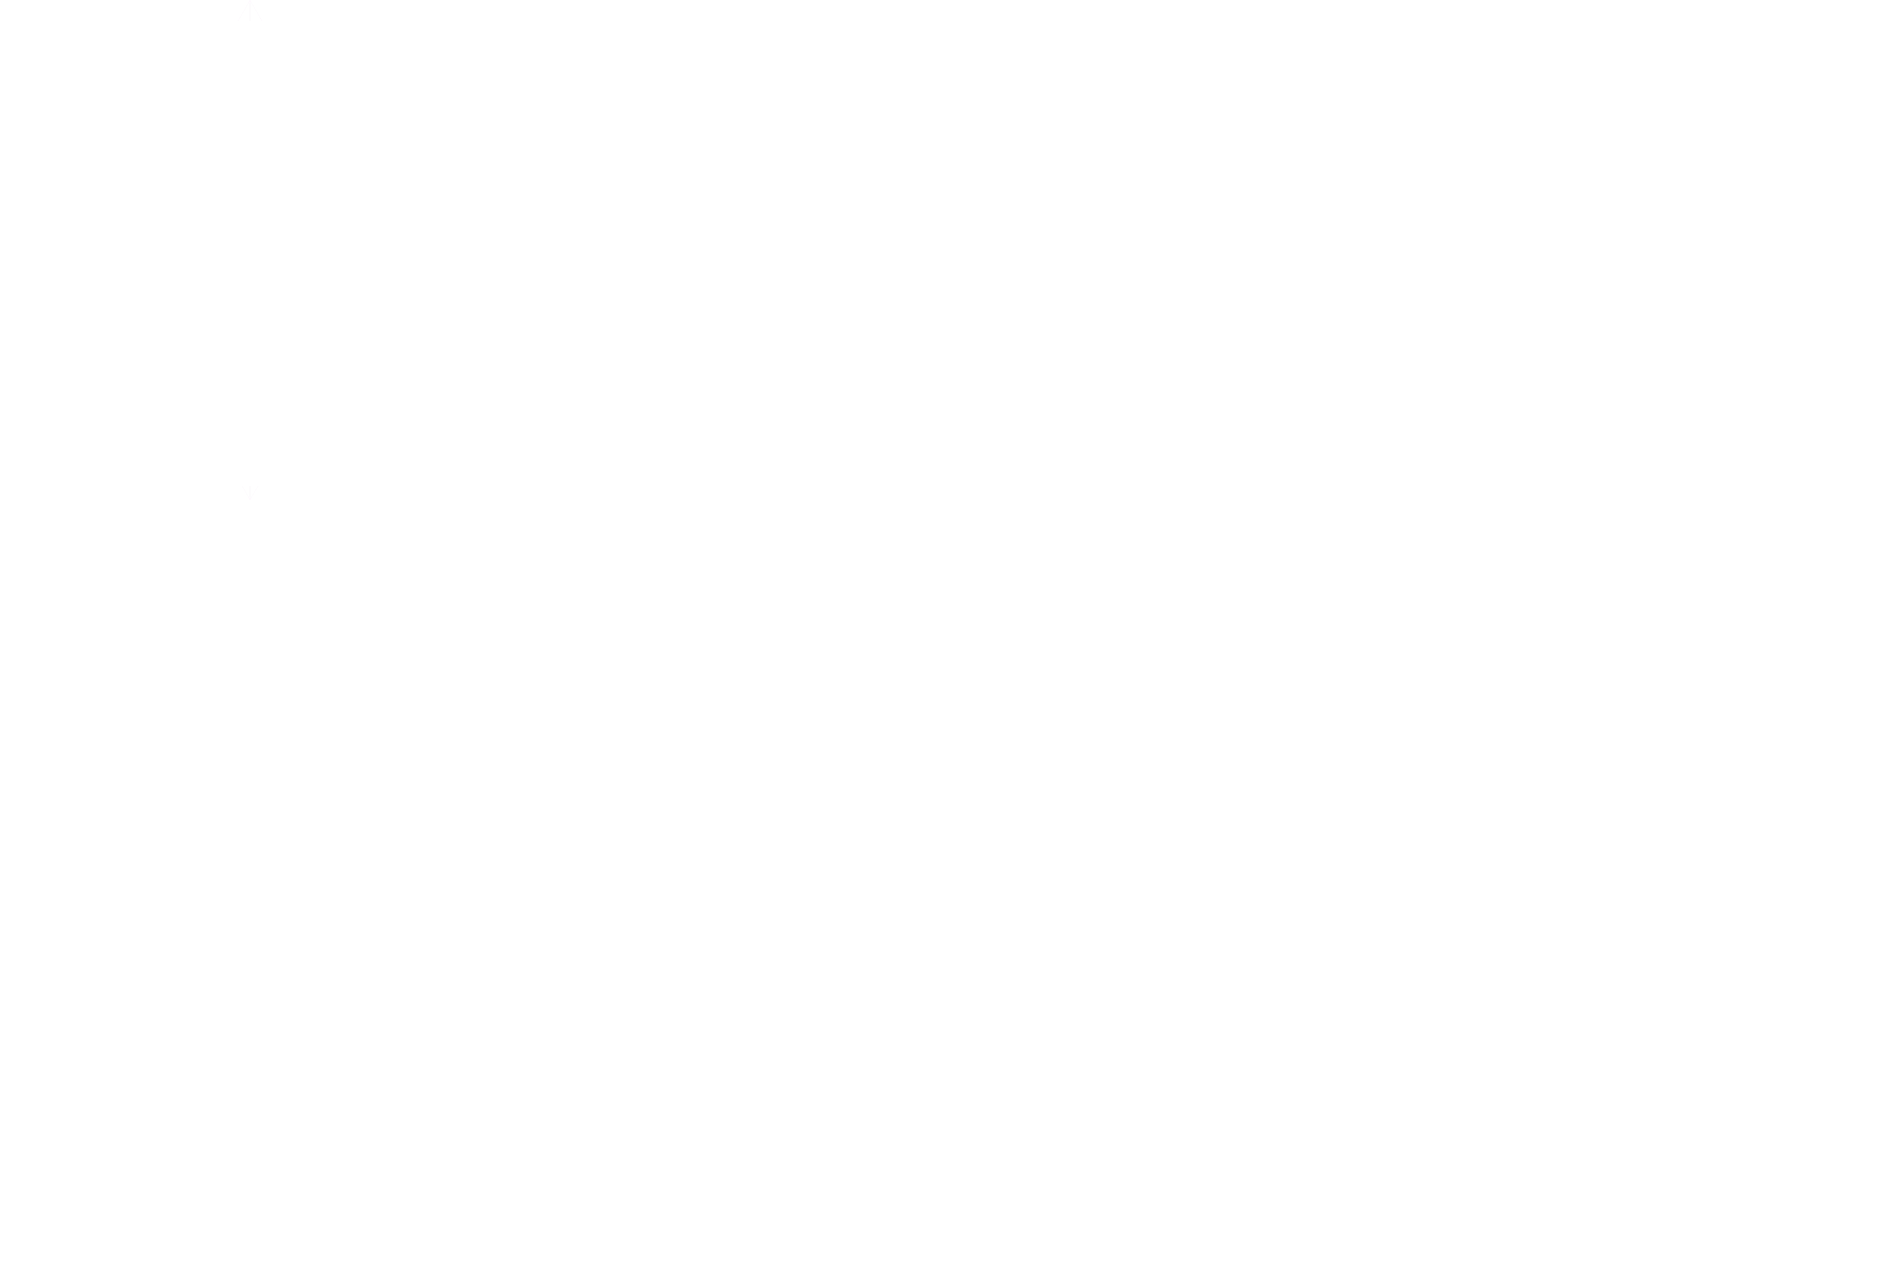
\includegraphics[keepaspectratio,scale=0.24]{images/title_logo}
		};
	\end{tikzpicture}
}
\setstretch{1.0}
\begin{frame}
\maketitle
\end{frame}
}

\begin{frame}[fragile]
\begin{center}
\begin{tabular}{c}
\begin{lstlisting}[basicstyle=\tiny,escapechar=!]
pragma experimental SMTChecker;

contract StateMachine {
    uint x;

    function f() public {
        if (x == 0)
            x = 1;
    }

    function g() public {
        if (x == 1)
            x = 0;
    }

    function invariant() public {
        !\color{mLightPurple}{assert(x <= 1);}!
    }
}
\end{lstlisting}
\end{tabular}
\end{center}
\end{frame}

\begin{frame}[fragile]
\begin{figure}
	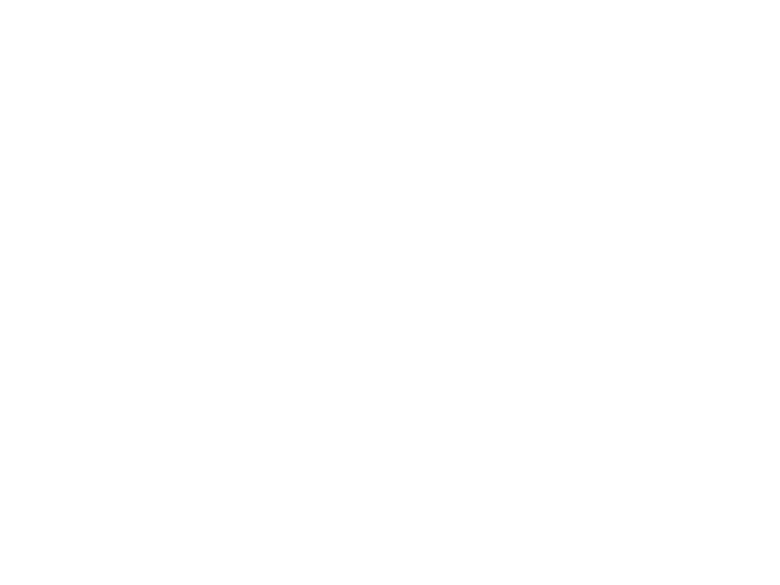
\includegraphics[scale=0.3]{images/state_machine}
\end{figure}
\end{frame}

\begin{frame}[fragile]
\begin{figure}
	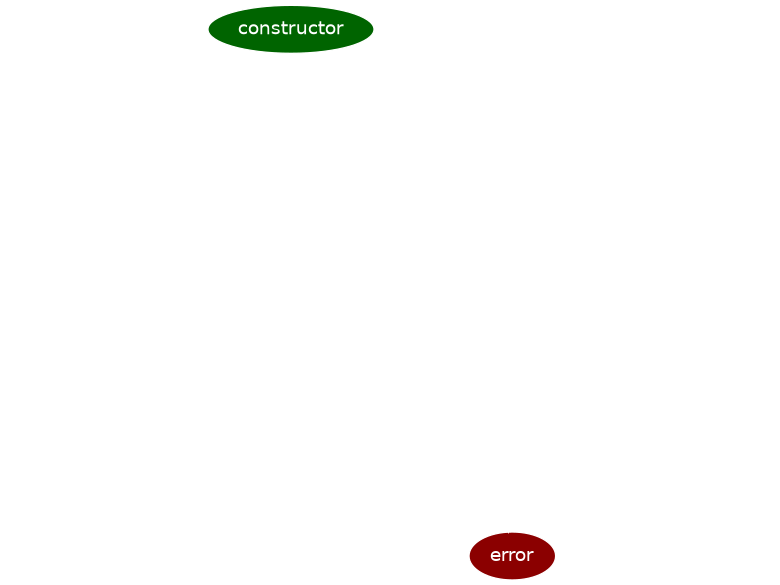
\includegraphics[scale=0.3]{images/state_machine_reachability}
\end{figure}
\end{frame}

\begin{frame}
Demo
\end{frame}

\begin{frame}[fragile]{}

\begin{figure}

\noindent\begin{minipage}{.49\textwidth}
Invariant: $x \le 2$
\begin{onlyenv}<2->
\begin{lstlisting}[basicstyle=\scriptsize,escapechar=!]
!\color{mLightPurple}{x <= 2;}!
f():
if (x == 0)
    x = 1;
!\color{mLightPurple}{x <= 2;}!
\end{lstlisting}
\end{onlyenv}

\begin{onlyenv}<4->
\begin{lstlisting}[basicstyle=\scriptsize,escapechar=!]
!\color{mLightPurple}{x <= 2;}!
g():
if (x == 1)
    x = 0;
!\color{mLightPurple}{x <= 2;}!
\end{lstlisting}
\end{onlyenv}

\begin{onlyenv}<6->
\begin{lstlisting}[basicstyle=\scriptsize,escapechar=!]
!\color{mLightPurple}{x <= 2;}!
h():
if (x == 7)
    x = 100;
!\color{mLightPurple}{x <= 2;}!
\end{lstlisting}
\end{onlyenv}

\end{minipage}
\noindent\begin{minipage}{.49\textwidth}
Invariant: $x \le 7$
\begin{onlyenv}<3->
\begin{lstlisting}[basicstyle=\scriptsize,escapechar=!]
!\color{mLightPurple}{x <= 7;}!
f():
if (x == 0)
    x = 1;
!\color{mLightPurple}{x <= 7;}!
\end{lstlisting}
\end{onlyenv}

\begin{onlyenv}<5->
\begin{lstlisting}[basicstyle=\scriptsize,escapechar=!]
!\color{mLightPurple}{x <= 7;}!
g():
if (x == 1)
    x = 0;
!\color{mLightPurple}{x <= 7;}!
\end{lstlisting}
\end{onlyenv}

\begin{onlyenv}<7->
\begin{lstlisting}[basicstyle=\scriptsize,escapechar=!]
!\color{mLightPurple}{x <= 7;}!
h():
if (x == 7)
    x = 100;
!\color{red}{x ? 7;}!
\end{lstlisting}
\end{onlyenv}

\end{minipage}
\end{figure}
\color{white}
\end{frame}

\begin{frame}
\begin{center}
$x \le 2$ is Inductive!\\
$x \le 2 \land \text{local behavior} \implies x \le 2$
\end{center}
\end{frame}

\begin{frame}{Inductive invariants}
	can summarize a relevant piece of code without relying on prior information
\end{frame}

\begin{frame}{Inductive invariants}
	are particularly useful to summarize the behavior of loops
\end{frame}

\begin{frame}
Demo
\end{frame}

\begin{frame}[fragile]{Loop invariants}
\begin{center}
\begin{tabular}{c}
\begin{lstlisting}[basicstyle=\small]
y = 0;
while (y < x)
    ++x;
assert(x == y);
\end{lstlisting}
\end{tabular}
\end{center}

\begin{itemize}
	\item $y \le x$ is the core property of the the loop
	\item After the loop, its condition is false: $y \ge x$
	\item Which leads to $y \le x \land y \ge x \implies y = x$.
\end{itemize}
\end{frame}

\begin{frame}{Inductive invariants}
	can also be applied to recursive programs,
	as the inductive hypothesis to be proven.
\end{frame}

\begin{frame}{How can we use inductive invariants for\\smart contract verification?}
	The lifecycle of a smart contract can also be seen as a control-flow containing a loop
\end{frame}

\begin{frame}[fragile]
\begin{figure}
	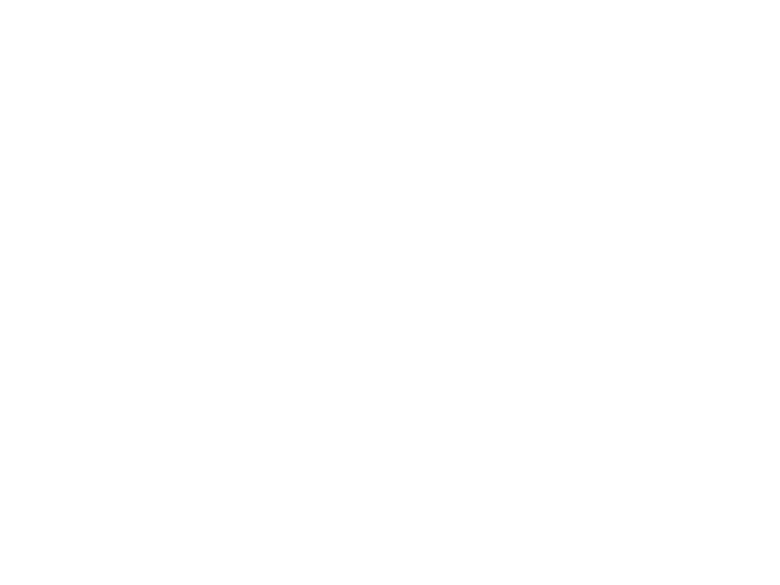
\includegraphics[scale=0.3]{images/state_machine}
\end{figure}
\end{frame}

\begin{frame}[fragile]
\begin{figure}
\noindent\begin{minipage}{.49\textwidth}
	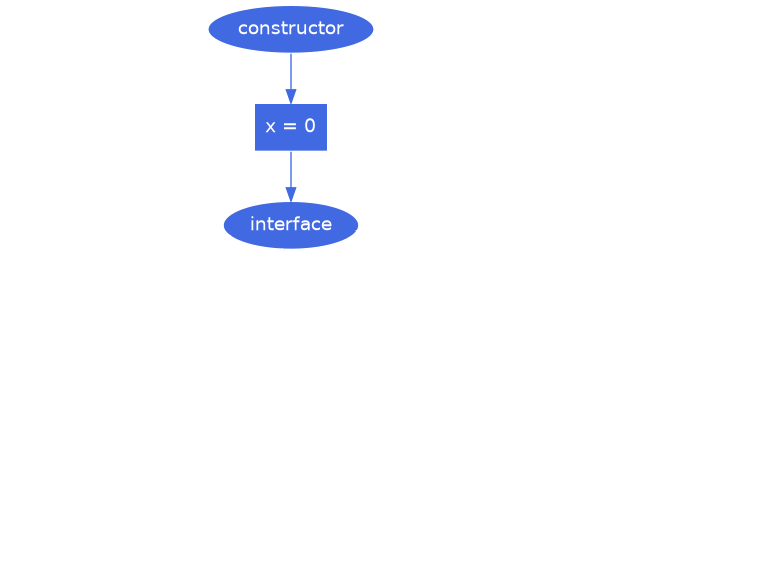
\includegraphics[scale=0.3]{images/state_machine_transition}
\end{minipage}
\noindent\begin{minipage}{.49\textwidth}
\begin{onlyenv}<2->
{\small
\begin{align*}
	\forall x \;\;\;\; {\only<4->{\color{mLightPurple}}constructor(x)} \land {\only<3-3>{\color{mLightPurple}}x = 0} \implies {\only<-2>{\color{mLightPurple}}interface(x)}\\
\end{align*}
}%
\end{onlyenv}
\end{minipage}
\end{figure}
\end{frame}

\begin{frame}[fragile]
\begin{figure}
\noindent\begin{minipage}{.49\textwidth}
	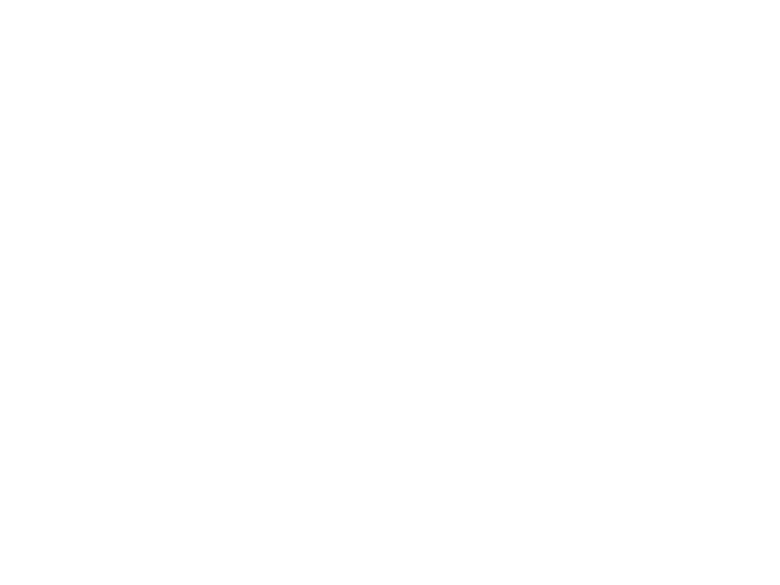
\includegraphics[scale=0.3]{images/state_machine}
\end{minipage}
\noindent\begin{minipage}{.49\textwidth}
{\small
\begin{align*}
	\forall x \;\;\;\; constructor(x)\\
	\forall x \;\;\;\; constructor(x) \land x = 0 \implies interface(x)\\
	\forall x \;\;\;\; interface(x) \implies f(x)\\
	\forall x \;\;\;\; interface(x) \implies g(x)\\
	\forall x \;\;\;\; interface(x) \implies invariant(x)\\
	\forall x \;\;\;\; f_{entry}(x) \land x = 0 \implies f_{body}(x)\\
	\forall x \;\;\;\; f_{body}(x) \land x' = 1 \implies f_{exit}(x')\\
	\forall x \;\;\;\; f_{entry}(x) \land x = 1 \implies f_{exit}(x)\\
	\forall x \;\;\;\; f_{exit}(x) \implies interface(x)\\
	\forall x \;\;\;\; invariant(x) \land x > 1 \implies error(x)\\
	\forall x \;\;\;\; invariant(x) \land x <= 1 \implies interface(x)
\end{align*}
}%
\end{minipage}
\end{figure}
\end{frame}

\begin{frame}[fragile]
\begin{figure}
\noindent\begin{minipage}{.49\textwidth}
	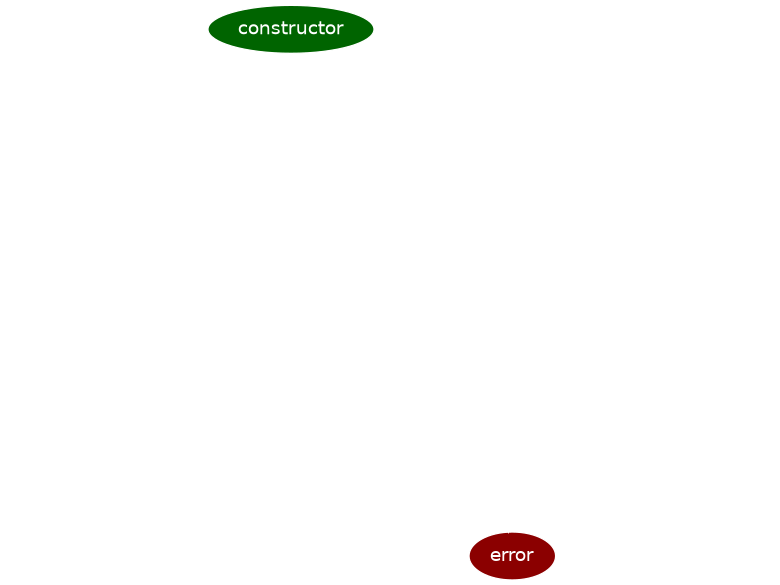
\includegraphics[scale=0.3]{images/state_machine_reachability}
\end{minipage}
\noindent\begin{minipage}{.49\textwidth}
{\small
\begin{align*}
	error(x) ?
\end{align*}
}%
\end{minipage}
\end{figure}
\end{frame}

\begin{frame}[fragile]
\begin{figure}
\noindent\begin{minipage}{.49\textwidth}
	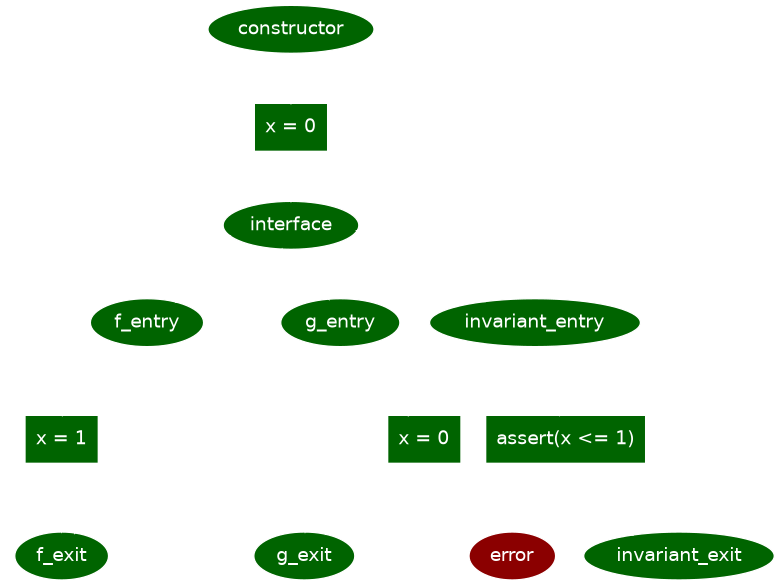
\includegraphics[scale=0.3]{images/state_machine_unreachable}
\end{minipage}
\noindent\begin{minipage}{.49\textwidth}
{\small
\begin{align*}
\forall x . error(x)\text{ is unreachable }
\end{align*}
}%
\end{minipage}
\end{figure}
\end{frame}

\begin{frame}
\begin{itemize}
	\item Existential positive Least Fixed-Point logic (E+LFP) matches Hoare logic\\Blass, A., Gurevich, Y.: Existential fixed-point logic. In: Computation Theory and Logic, In Memory of Dieter Rödding. pp. 20–36 (1987)
	\item E+LFP solved by CHCs satisfiability\\Bjørner, N., Gurfinkel, A., McMillan, K.L., Rybalchenko, A.: Horn clause solvers for program verification. In: Fields of Logic and Computation II. pp. 24–51 (2015)
\end{itemize}
\end{frame}

\begin{frame}[fragile]
\begin{figure}
\noindent\begin{minipage}{.49\textwidth}
	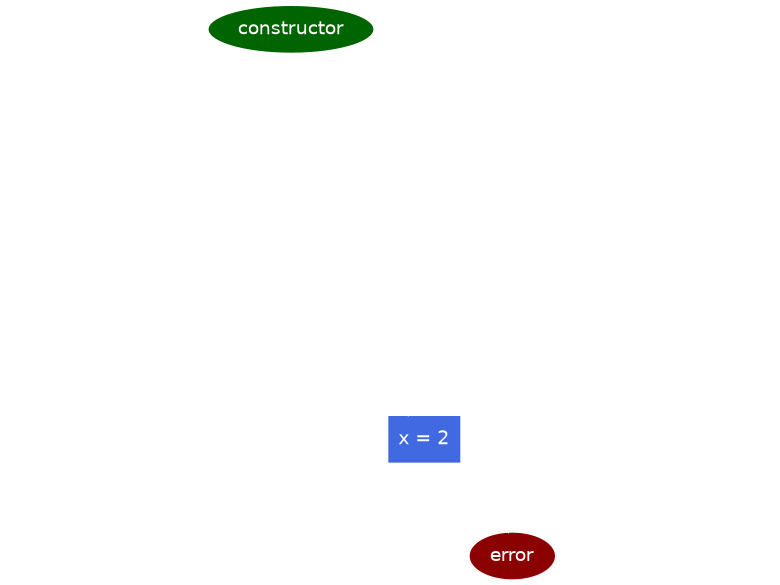
\includegraphics[scale=0.3]{images/state_machine_counterexample}
\end{minipage}
\noindent\begin{minipage}{.49\textwidth}
{\small
\begin{align*}
	error(x) ?
\end{align*}
}%
\end{minipage}
\end{figure}
\end{frame}

\begin{frame}
Demo
\end{frame}

\begin{frame}[fragile]
\begin{figure}
\noindent\begin{minipage}{.49\textwidth}
	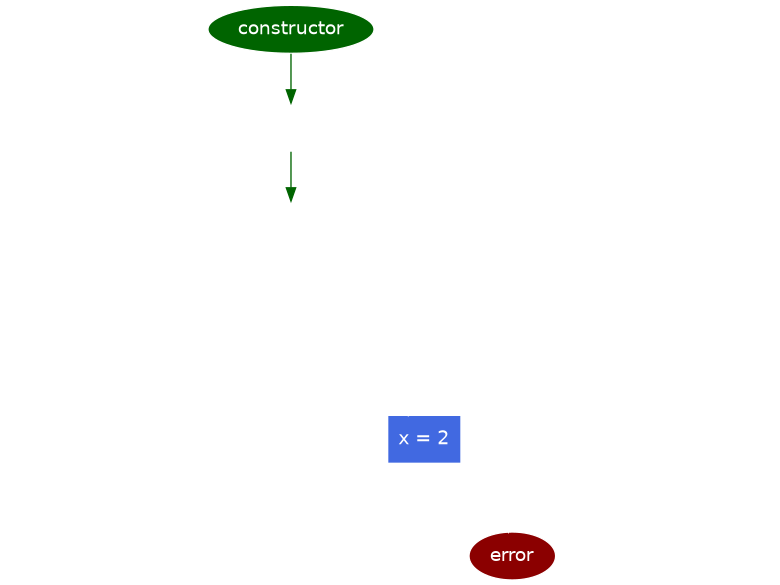
\includegraphics[scale=0.3]{images/state_machine_counterexample_path_constructor}
\end{minipage}
\noindent\begin{minipage}{.49\textwidth}
{\small
\begin{align*}
	error(x) ?
\end{align*}
}%
\end{minipage}
\end{figure}
\end{frame}

\begin{frame}[fragile]
\begin{figure}
\noindent\begin{minipage}{.49\textwidth}
	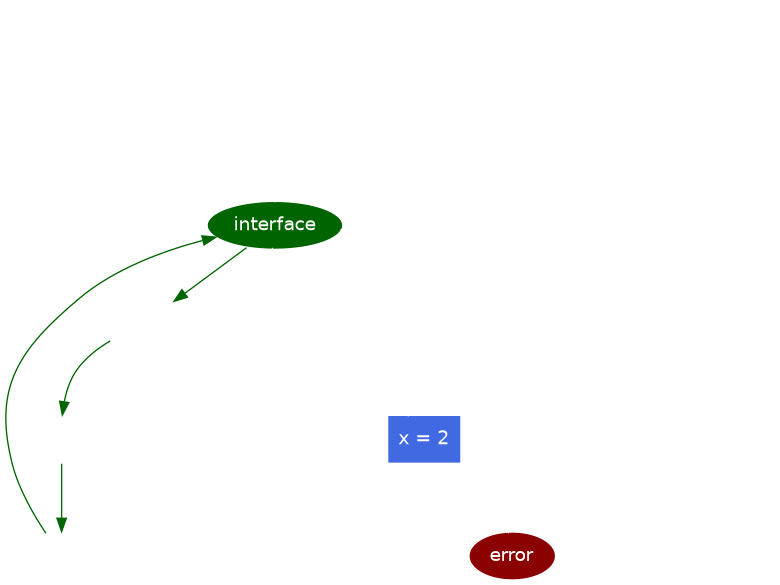
\includegraphics[scale=0.3]{images/state_machine_counterexample_path_1}
\end{minipage}
\noindent\begin{minipage}{.49\textwidth}
{\small
\begin{align*}
	error(x) ?
\end{align*}
}%
\end{minipage}
\end{figure}
\end{frame}

\begin{frame}[fragile]
\begin{figure}
\noindent\begin{minipage}{.49\textwidth}
	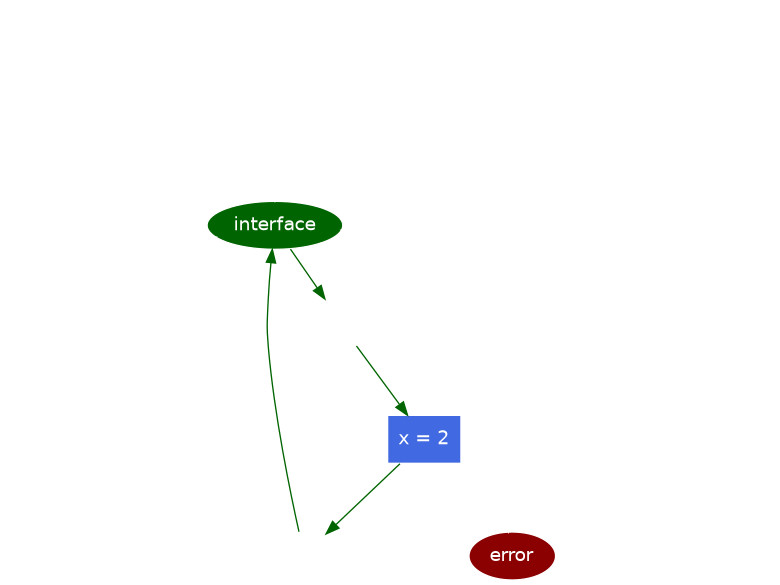
\includegraphics[scale=0.3]{images/state_machine_counterexample_path_2}
\end{minipage}
\noindent\begin{minipage}{.49\textwidth}
{\small
\begin{align*}
	error(x) ?
\end{align*}
}%
\end{minipage}
\end{figure}
\end{frame}

\begin{frame}[fragile]
\begin{figure}
\noindent\begin{minipage}{.49\textwidth}
	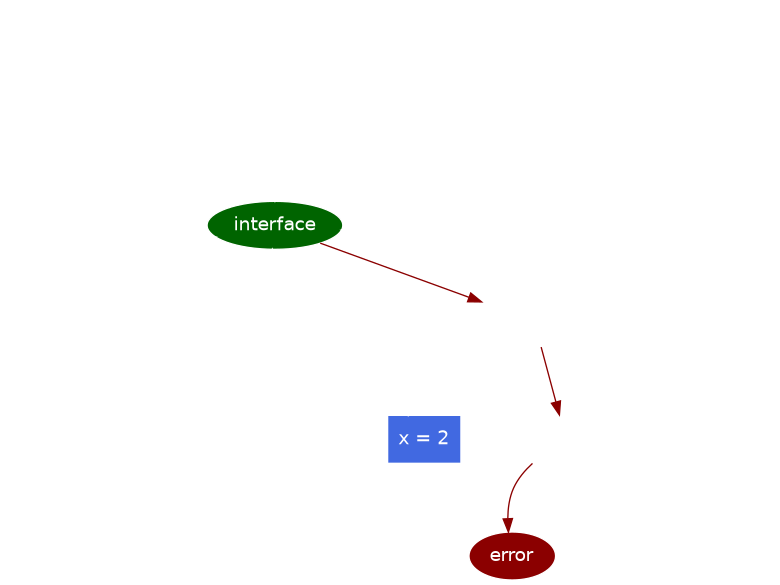
\includegraphics[scale=0.3]{images/state_machine_counterexample_path_3}
\end{minipage}
\noindent\begin{minipage}{.49\textwidth}
{\small
	error(x) is reachable!
}%
\end{minipage}
\end{figure}
The sequence that leads to the error is\\
deployment, f(), g(), invariant().
\end{frame}

\begin{frame}{Horn solvers}
\begin{itemize}
	\item Predicate abstraction
	\item Abstract interpretation
	\item Maximal inductive subsets
	\item Machine learning
\end{itemize}
\end{frame}

\begin{frame}{Horn solvers}
\begin{itemize}
	\item SMT-based unbounded model checking - PDR/IC3
	\item Spacer - spacer.bitbucket.io
	\item Backwards reachability
	\item Quantifier-free SMT queries and interpolation to find predecessors and new lemmas
\end{itemize}
\end{frame}

\begin{frame}{What's next}
\begin{itemize}
	\item Function calls!
	\begin{itemize}
		\item Function summaries
		\item No changes in the state of the caller contract
		\item Synthesis of external functions
		\item Multi-contract-unbounded-transactions properties
		\item Maybe entire state?
	\end{itemize}
	\item Nice looking counterexamples and invariants
	\item Better usability
	\item Simple formal spec language - github.com/ethereum/smart-contract-spec-lang
\end{itemize}
\end{frame}

\begin{frame}{Final remarks}
\begin{itemize}
	\item SMT solvers are powerful and fast (hopefully as powerful as we sell them)
	\item Unbounded model checking with PDR
	\item Unbounded transaction properties and counterexamples
	\item Embedded in the Solidity compiler
	\item Contract inductive invariants can further help verification of bytecode (added lemmas)
\end{itemize}
\end{frame}

\begin{frame}[standout,fragile]
\begin{center}
Thank you!
\end{center}
\end{frame}
 
\end{document}
